\documentclass[12pt,a4paper]{article}
\usepackage{amsmath, amssymb, geometry, booktabs, xcolor, hyperref,
            listings, pgfplots, tcolorbox, enumitem, fancyhdr, tikz, array}
\usepgfplotslibrary{fillbetween}
\geometry{margin=2.5cm}
\pgfplotsset{compat=1.18}
\tcbuselibrary{skins, breakable}

% Define custom environments
\newtcolorbox{curiositybox}[1]{colback=yellow!10, colframe=orange!80, title=#1, breakable}
\newtcolorbox{infobox}[1]{colback=blue!5, colframe=blue!60, title=#1, breakable}
\newtcolorbox{mistakebox}[1]{colback=red!5, colframe=red!60, title=#1, breakable}
\newtcolorbox{learnbox}[1]{colback=green!5, colframe=green!60, title=#1, breakable}

% Header and Footer
\pagestyle{fancy}
\fancyhf{}
\lhead{Differential Calculus of Several Variables}
\rhead{Unit 4 -- LAC}
\cfoot{\thepage}

% Document Title Setup
\title{\textbf{Differential Calculus of Several Variables} \\ \large Unit 4 -- Multivariable Differentiation and Optimization}
\author{Department of Mathematics}
\date{\today}

\begin{document}
\maketitle
\tableofcontents
\newpage

%===========================================================
\section{Real-World Engineering Hook}
%===========================================================

\begin{curiositybox}{Why Should an Engineer Care?}
Imagine you are running a Finite Element Method (FEM) simulation to model heat distribution in a steel turbine blade. The temperature field \(T(x, y, z)\) assigns a temperature value to every point in the blade. The heat flux---the rate at which heat flows through the material---is determined entirely by the partial derivatives \(\frac{\partial T}{\partial x}\), \(\frac{\partial T}{\partial y}\), and \(\frac{\partial T}{\partial z}\). If these partial derivatives are large in a particular region, the blade will experience severe thermal gradients that can cause fatigue cracking.

Now suppose the temperature function \(T(x,y,z)\) is \textbf{not continuous} at some interior point---perhaps because of a modelling error or a badly meshed region. The limit of \(T\) as you approach that point depends on the direction you come from, meaning the solver gets different temperature values depending on which element it queries. The FEM solver diverges, producing garbage output. Engineers call this a ``thermal shock'' instability in the mesh.

Understanding limits, continuity, and partial derivatives in multiple variables is not optional mathematics---it is the foundation on which every numerical simulation, every optimization algorithm, and every sensitivity analysis in engineering is built. From aerodynamic pressure fields over a wing to stress distributions in a bridge, multivariable calculus is the language the physical world speaks.
\end{curiositybox}

%===========================================================
\section{Why This Topic Exists}
%===========================================================

The move from single-variable calculus to multivariable calculus is not merely adding more variables. It introduces fundamentally new phenomena: limits can fail to exist even when they exist along every straight-line path; partial derivatives can exist everywhere without the function being differentiable; and the chain rule branches into a network of dependencies rather than a single chain.

\begin{center}
\begin{tabular}{@{}lll@{}}
\toprule
\textbf{Sub-Topic} & \textbf{Core Theory} & \textbf{Engineering Consequence} \\
\midrule
Functions, Limits \& Continuity & Path-independent limits, \(\epsilon\text{-}\delta\) definition & FEM mesh stability, sensor field interpolation \\
Partial Derivatives (1st \& 2nd order) & \(\frac{\partial f}{\partial x}\), Clairaut's theorem & Heat flux computation, stress tensor components \\
Total Derivative \& Chain Rule & \(df = \frac{\partial f}{\partial x}dx + \frac{\partial f}{\partial y}dy\), implicit diff. & Sensitivity analysis, error propagation in measurements \\
\bottomrule
\end{tabular}
\end{center}

\begin{learnbox}{Core Learning Objectives}
By the end of this topic you will be able to:
\begin{itemize}
  \item Define and evaluate limits of functions of two variables, verifying path-independence.
  \item Check continuity of a multivariable function at a given point.
  \item Compute first- and second-order partial derivatives and verify Clairaut's theorem.
  \item Write the total differential and apply the multivariable chain rule.
  \item Perform implicit differentiation using the total derivative.
  \item Interpret partial and total derivatives geometrically and in engineering contexts.
\end{itemize}
\end{learnbox}

%===========================================================
\section{Intuition First and Mathematical Definitions}
%===========================================================

\subsection{Functions of Several Variables, Limits and Continuity}

Think of a function of two variables \(f(x,y)\) as a machine that takes a pair of real numbers and returns a single real number---like reading the temperature at coordinates \((x,y)\) on a flat plate. Unlike the single-variable case, where you approach a point from only two directions (left and right), in two dimensions you can approach \((a,b)\) along infinitely many paths: straight lines at any angle, parabolas, spirals, and more. The limit must be the same along \emph{every} one of these paths for it to exist.

\begin{infobox}{Functions of Several Variables, Limits and Continuity}
\textbf{Definition (Function of Two Variables):} A function \(f: D \subseteq \mathbb{R}^2 \to \mathbb{R}\) assigns to each point \((x,y)\) in domain \(D\) a unique real number \(f(x,y)\). The \textit{domain} is the set of all \((x,y)\) for which \(f\) is defined.

\textbf{Level Curves:} The set \(\{(x,y) \mid f(x,y) = c\}\) for constant \(c\) is called a level curve of \(f\). Level curves are the 2D projections of the 3D surface \(z = f(x,y)\).

\textbf{Limit (\(\epsilon\text{-}\delta\) Definition):}
\[
\lim_{(x,y)\to(a,b)} f(x,y) = L
\]
if and only if for every \(\epsilon > 0\) there exists \(\delta > 0\) such that
\[
0 < \sqrt{(x-a)^2+(y-b)^2} < \delta \implies |f(x,y)-L| < \epsilon.
\]

\textbf{Non-Existence of a Limit:} If \(f\) approaches different values \(L_1 \neq L_2\) along two different paths to \((a,b)\), then the limit does not exist.

\textbf{Continuity:} \(f\) is continuous at \((a,b)\) if:
\begin{enumerate}
  \item \(f(a,b)\) is defined,
  \item \(\lim_{(x,y)\to(a,b)} f(x,y)\) exists,
  \item \(\lim_{(x,y)\to(a,b)} f(x,y) = f(a,b)\).
\end{enumerate}

\textbf{Algebra of Limits:} If \(\lim f = L\) and \(\lim g = M\), then \(\lim (f+g) = L+M\), \(\lim (fg) = LM\), and \(\lim (f/g) = L/M\) provided \(M \neq 0\).
\end{infobox}

\textbf{Worked Example 1.1 --- Limit exists (path-independent):}

Evaluate \(\displaystyle\lim_{(x,y)\to(1,2)} (3x^2 + 2y)\).

\textit{Step 1: Check if the function is a polynomial.}
\(f(x,y) = 3x^2 + 2y\) is a polynomial in \(x\) and \(y\). Polynomials are continuous everywhere on \(\mathbb{R}^2\).

\textit{Step 2: Substitute directly.}
\[
\lim_{(x,y)\to(1,2)} (3x^2+2y) = 3(1)^2 + 2(2) = 3 + 4 = 7.
\]
The limit is \(7\) regardless of the path taken to \((1,2)\).

\textbf{Worked Example 1.2 --- Limit does not exist (path-dependent):}

Evaluate \(\displaystyle\lim_{(x,y)\to(0,0)} \frac{xy}{x^2+y^2}\).

\textit{Step 1: Path 1 --- along \(y = 0\).}
\[
f(x,0) = \frac{x \cdot 0}{x^2+0} = \frac{0}{x^2} = 0 \quad (x \neq 0).
\]
Limit along this path: \(0\).

\textit{Step 2: Path 2 --- along \(y = x\).}
\[
f(x,x) = \frac{x \cdot x}{x^2+x^2} = \frac{x^2}{2x^2} = \frac{1}{2} \quad (x \neq 0).
\]
Limit along this path: \(\dfrac{1}{2}\).

\textit{Step 3: Conclude.}
Since \(0 \neq \dfrac{1}{2}\), the limit does not exist at \((0,0)\).

%-----------------------------------------------------------
\subsection{Partial Derivatives and Higher-Order Partial Derivatives}

Imagine holding all variables fixed except one and asking: ``how fast does \(f\) change in this one direction?'' That is a partial derivative. It is exactly a single-variable derivative in disguise---you freeze every variable except the one you are differentiating with respect to. Second-order partials measure how the rate of change itself changes, forming the entries of the \textit{Hessian matrix} used in optimization.

\begin{infobox}{Partial Derivatives and Higher-Order Partial Derivatives}
\textbf{First-Order Partial Derivatives (defined as limits):}
\[
\frac{\partial f}{\partial x}(a,b) = \lim_{h \to 0} \frac{f(a+h,\, b) - f(a,b)}{h},
\]
\[
\frac{\partial f}{\partial y}(a,b) = \lim_{k \to 0} \frac{f(a,\, b+k) - f(a,b)}{k}.
\]
Notations: \(f_x,\; f_y,\; \partial f/\partial x,\; \partial f/\partial y\).

\textbf{Second-Order Partial Derivatives:}
\[
f_{xx} = \frac{\partial^2 f}{\partial x^2}, \quad
f_{yy} = \frac{\partial^2 f}{\partial y^2}, \quad
f_{xy} = \frac{\partial^2 f}{\partial x \partial y} = \frac{\partial}{\partial x}\!\left(\frac{\partial f}{\partial y}\right), \quad
f_{yx} = \frac{\partial^2 f}{\partial y \partial x} = \frac{\partial}{\partial y}\!\left(\frac{\partial f}{\partial x}\right).
\]

\textbf{Clairaut's Theorem (Symmetry of Mixed Partials):} If \(f_{xy}\) and \(f_{yx}\) are both continuous on an open disk around \((a,b)\), then
\[
f_{xy}(a,b) = f_{yx}(a,b).
\]

\textbf{Partial Derivative Rules:} Treat all other variables as constants and apply the standard single-variable differentiation rules (product rule, chain rule, quotient rule).

\textbf{Gradient Vector:}
\[
\nabla f(x,y) = \left(\frac{\partial f}{\partial x},\; \frac{\partial f}{\partial y}\right).
\]
The gradient points in the direction of steepest ascent of \(f\).
\end{infobox}

\textbf{Worked Example 2.1 --- All second-order partial derivatives and Clairaut verification:}

Let \(f(x,y) = x^3 y^2 - 2x^2 y + y^3\).

\textit{Step 1: First-order partial derivatives.}
\begin{align*}
f_x &= \frac{\partial}{\partial x}(x^3 y^2 - 2x^2 y + y^3) = 3x^2 y^2 - 4xy, \\
f_y &= \frac{\partial}{\partial y}(x^3 y^2 - 2x^2 y + y^3) = 2x^3 y - 2x^2 + 3y^2.
\end{align*}

\textit{Step 2: Second-order partials.}
\begin{align*}
f_{xx} &= \frac{\partial}{\partial x}(3x^2 y^2 - 4xy) = 6xy^2 - 4y, \\
f_{yy} &= \frac{\partial}{\partial y}(2x^3 y - 2x^2 + 3y^2) = 2x^3 + 6y, \\
f_{xy} &= \frac{\partial}{\partial y}(3x^2 y^2 - 4xy) = 6x^2 y - 4x, \\
f_{yx} &= \frac{\partial}{\partial x}(2x^3 y - 2x^2 + 3y^2) = 6x^2 y - 4x.
\end{align*}

\textit{Step 3: Verify Clairaut's theorem.}
\[
f_{xy} = 6x^2 y - 4x = f_{yx}. \quad \checkmark
\]
The mixed partials are identical, confirming Clairaut's theorem. Note that all second-order partials of a polynomial are continuous everywhere, so the theorem applies.

%-----------------------------------------------------------
\subsection{Total Derivative and Chain Rule}

The partial derivatives \(f_x\) and \(f_y\) each capture change in one direction. The \textit{total differential} assembles them into a single linear approximation that captures the change in \(f\) due to simultaneous small changes in both \(x\) and \(y\). When \(x\) and \(y\) are themselves functions of another variable (e.g., time \(t\) along a path), the chain rule propagates rates of change through the network of dependencies.

\begin{infobox}{Total Derivative and Chain Rule}
\textbf{Total Differential:} If \(f(x,y)\) has continuous partial derivatives, the total differential is
\[
df = \frac{\partial f}{\partial x}\,dx + \frac{\partial f}{\partial y}\,dy.
\]
This is the best linear approximation of the change in \(f\) when \(x\) changes by \(dx\) and \(y\) changes by \(dy\).

\textbf{Chain Rule (Case 1 --- one parameter):} If \(z = f(x,y)\) and \(x = x(t)\), \(y = y(t)\), then
\[
\frac{dz}{dt} = \frac{\partial f}{\partial x}\frac{dx}{dt} + \frac{\partial f}{\partial y}\frac{dy}{dt}.
\]

\textbf{Chain Rule (Case 2 --- two parameters):} If \(z = f(x,y)\) and \(x = x(s,t)\), \(y = y(s,t)\), then
\[
\frac{\partial z}{\partial s} = \frac{\partial f}{\partial x}\frac{\partial x}{\partial s} + \frac{\partial f}{\partial y}\frac{\partial y}{\partial s}, \qquad
\frac{\partial z}{\partial t} = \frac{\partial f}{\partial x}\frac{\partial x}{\partial t} + \frac{\partial f}{\partial y}\frac{\partial y}{\partial t}.
\]

\textbf{Implicit Differentiation:} If \(F(x,y) = 0\) defines \(y\) implicitly as a function of \(x\), then
\[
\frac{dy}{dx} = -\frac{F_x}{F_y}, \quad \text{provided } F_y \neq 0.
\]
This follows directly from the total differential: \(dF = F_x\,dx + F_y\,dy = 0\).

\textbf{Linear Approximation:} Near the point \((a,b)\),
\[
f(x,y) \approx f(a,b) + f_x(a,b)(x-a) + f_y(a,b)(y-b).
\]
\end{infobox}

\textbf{Worked Example 3.1 --- Chain rule along a path:}

Let \(z = f(x,y) = x^2 y + \sin(xy)\), where \(x = e^t\) and \(y = t^2\). Find \(\dfrac{dz}{dt}\) at \(t = 0\).

\textit{Step 1: Compute partial derivatives.}
\begin{align*}
f_x &= 2xy + y\cos(xy), \\
f_y &= x^2 + x\cos(xy).
\end{align*}

\textit{Step 2: Compute derivatives of \(x\) and \(y\) with respect to \(t\).}
\[
\frac{dx}{dt} = e^t, \qquad \frac{dy}{dt} = 2t.
\]

\textit{Step 3: Apply the chain rule.}
\[
\frac{dz}{dt} = f_x \cdot \frac{dx}{dt} + f_y \cdot \frac{dy}{dt}
= (2xy + y\cos(xy)) e^t + (x^2 + x\cos(xy)) \cdot 2t.
\]

\textit{Step 4: Evaluate at \(t = 0\). At \(t=0\): \(x = e^0 = 1\), \(y = 0^2 = 0\).}
\begin{align*}
f_x(1,0) &= 2(1)(0) + 0\cdot\cos(0) = 0, \\
f_y(1,0) &= 1^2 + 1\cdot\cos(0) = 1 + 1 = 2, \\
\frac{dx}{dt}\big|_{t=0} &= e^0 = 1, \quad \frac{dy}{dt}\big|_{t=0} = 0.
\end{align*}
\[
\left.\frac{dz}{dt}\right|_{t=0} = 0 \cdot 1 + 2 \cdot 0 = 0.
\]

\textbf{Worked Example 3.2 --- Implicit differentiation:}

Given \(F(x,y) = x^3 + y^3 - 6xy = 0\) (folium of Descartes), find \(\dfrac{dy}{dx}\).

\textit{Step 1: Compute \(F_x\) and \(F_y\).}
\[
F_x = 3x^2 - 6y, \qquad F_y = 3y^2 - 6x.
\]

\textit{Step 2: Apply the implicit differentiation formula.}
\[
\frac{dy}{dx} = -\frac{F_x}{F_y} = -\frac{3x^2 - 6y}{3y^2 - 6x} = \frac{6y - 3x^2}{3y^2 - 6x} = \frac{2y - x^2}{y^2 - 2x}.
\]

%===========================================================
\section{Visual Artifacts and Geometric Interpretation}
%===========================================================

\subsection*{4.1 --- 3D Surface Plot of \(z = x^2 + y^2\)}

\begin{center}
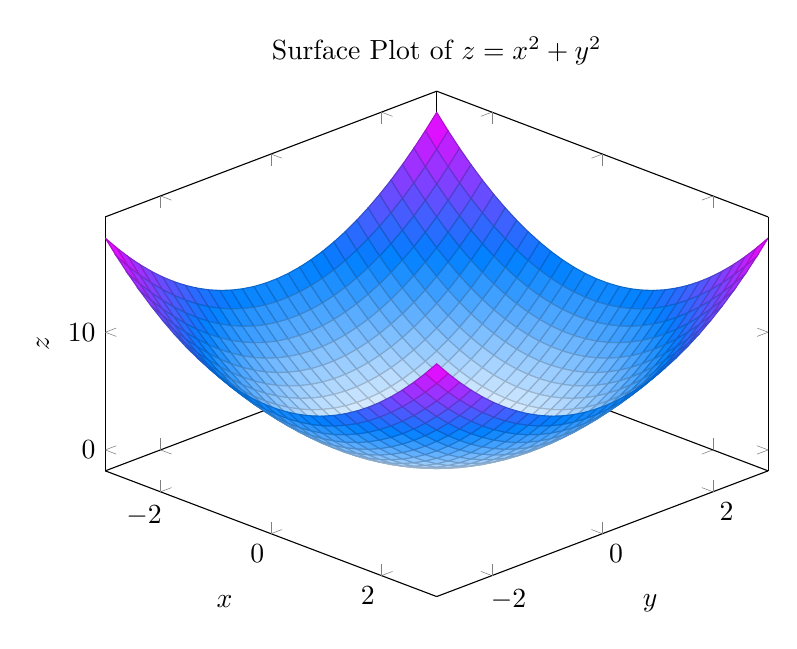
\begin{tikzpicture}
\begin{axis}[
    title={Surface Plot of $z = x^2 + y^2$},
    xlabel={$x$},
    ylabel={$y$},
    zlabel={$z$},
    colormap/cool,
    width=10cm, height=8cm,
    view={45}{35}
]
\addplot3[surf, samples=30, domain=-3:3]
    {x^2 + y^2};
\end{axis}
\end{tikzpicture}
\end{center}

\subsection*{4.2 --- Level Curves (Contour Plot) of \(f(x,y) = x^2 + y^2\)}

\begin{center}
\begin{tikzpicture}
\begin{axis}[
    title={Level Curves of $f(x,y) = x^2 + y^2$},
    xlabel={$x$},
    ylabel={$y$},
    width=9cm, height=8cm,
    view={0}{90}
]
\addplot3[contour gnuplot={levels={1,4,9,16,25}}, samples=40, domain=-6:6]
    {x^2 + y^2};
\end{axis}
\end{tikzpicture}
\end{center}

\subsection*{4.3 --- Gradient Vector Direction at a Point}

\begin{center}
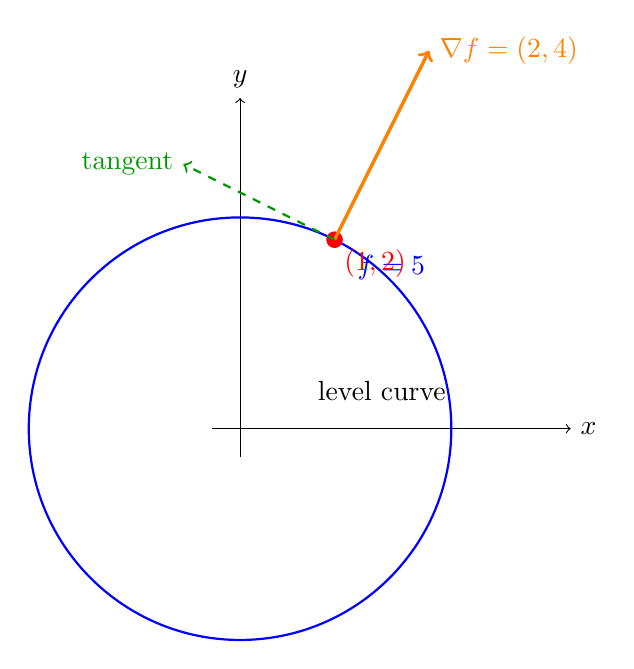
\begin{tikzpicture}[scale=1.2]
  % Axes
  \draw[->] (-0.3,0) -- (3.5,0) node[right] {$x$};
  \draw[->] (0,-0.3) -- (0,3.5) node[above] {$y$};
  % Level curve (circle) at f=5 for f=x^2+y^2
  \draw[blue, thick] (0,0) circle (2.236cm);
  \node[blue] at (1.6,1.7) {$f=5$};
  % Point on level curve at (1,2)
  \fill[red] (1,2) circle (2.5pt) node[below right] {$(1,2)$};
  % Gradient vector: nabla f = (2x, 2y) = (2,4) at (1,2), scaled to 0.5
  \draw[->, very thick, orange] (1,2) -- (2,4) node[right] {$\nabla f = (2,4)$};
  % Tangent to level curve (perpendicular to gradient): direction (-4,2), scaled to 0.4
  \draw[->, thick, green!60!black, dashed] (1,2) -- (-0.6,2.8) node[left] {tangent};
  \node at (1.5,0.4) {level curve};
\end{tikzpicture}
\end{center}

The gradient \(\nabla f\) at any point is always perpendicular to the level curve through that point and points in the direction of steepest increase of \(f\).

%===========================================================
\section{Step-by-Step Algorithmic Workflow}
%===========================================================

\subsection*{Workflow A: Checking Whether a Limit Exists}

\begin{enumerate}
  \item \textbf{Simplify:} Check if \(f(x,y)\) is a polynomial or composed of continuous functions. If yes, substitute directly.
  \item \textbf{Path 1 --- Along \(y=0\):} Substitute \(y=0\), simplify, take \(x \to a\). Record limit \(L_1\).
  \item \textbf{Path 2 --- Along \(x=0\):} Substitute \(x=0\), simplify, take \(y \to b\). Record limit \(L_2\).
  \item \textbf{Path 3 --- Along \(y=mx\):} Substitute \(y=mx\) for general \(m\), take \(x \to 0\). If the result depends on \(m\), the limit does not exist.
  \item \textbf{Path 4 (if needed) --- Along \(y=x^2\):} Substitute \(y=x^2\), take \(x \to 0\).
  \item \textbf{Conclusion:} If all paths give the same value \(L\), the limit is likely \(L\) (verify using squeeze theorem if needed). If any two paths give different values, the limit does not exist.
\end{enumerate}

\subsection*{Workflow B: Computing All Partial Derivatives up to Order 2}

\begin{enumerate}
  \item \textbf{Compute \(f_x\):} Treat \(y\) as a constant; differentiate with respect to \(x\).
  \item \textbf{Compute \(f_y\):} Treat \(x\) as a constant; differentiate with respect to \(y\).
  \item \textbf{Compute \(f_{xx}\):} Differentiate \(f_x\) again with respect to \(x\).
  \item \textbf{Compute \(f_{yy}\):} Differentiate \(f_y\) again with respect to \(y\).
  \item \textbf{Compute \(f_{xy}\):} Differentiate \(f_x\) with respect to \(y\).
  \item \textbf{Compute \(f_{yx}\):} Differentiate \(f_y\) with respect to \(x\).
  \item \textbf{Verify:} Check that \(f_{xy} = f_{yx}\) (Clairaut's theorem, valid when both are continuous).
\end{enumerate}

\subsection*{Workflow C: Applying the Chain Rule Step-by-Step}

\begin{enumerate}
  \item \textbf{Identify the outer function:} Write \(z = f(x,y)\). Note all variables \(x\) and \(y\) depend on.
  \item \textbf{Compute partial derivatives:} Find \(f_x\) and \(f_y\).
  \item \textbf{Compute inner derivatives:} Find \(dx/dt\) and \(dy/dt\) (or \(\partial x/\partial s\), etc.).
  \item \textbf{Multiply and add:} Apply \(\dfrac{dz}{dt} = f_x \dfrac{dx}{dt} + f_y \dfrac{dy}{dt}\).
  \item \textbf{Substitute:} Replace \(x(t)\) and \(y(t)\) before evaluating at a specific \(t\) if required.
  \item \textbf{Simplify:} Collect terms and simplify the final expression.
\end{enumerate}

%===========================================================
\section{Fully Worked Step-by-Step Numerical Examples}
%===========================================================

\textbf{Example 1 --- Limit does not exist:}

Evaluate \(\displaystyle\lim_{(x,y)\to(0,0)} \frac{xy}{x^2+y^2}\).

\textit{Path 1: Along \(y=0\).}
\[
\lim_{x\to 0} \frac{x \cdot 0}{x^2 + 0} = \lim_{x\to 0} 0 = 0.
\]

\textit{Path 2: Along \(y=x\).}
\[
\lim_{x\to 0} \frac{x \cdot x}{x^2 + x^2} = \lim_{x\to 0} \frac{x^2}{2x^2} = \lim_{x\to 0} \frac{1}{2} = \frac{1}{2}.
\]

\textit{Path 3: Along \(y = mx\) for general slope \(m\).}
\[
\lim_{x\to 0} \frac{x \cdot mx}{x^2 + m^2 x^2} = \lim_{x\to 0} \frac{mx^2}{(1+m^2)x^2} = \frac{m}{1+m^2}.
\]
This result depends on \(m\). For example, \(m=0\) gives \(0\) and \(m=1\) gives \(\dfrac{1}{2}\).

\textit{Conclusion:} The limit depends on the path and therefore \textbf{does not exist}.

\bigskip

\textbf{Example 2 --- All second-order partial derivatives and Clairaut's theorem:}

Let \(f(x,y) = x^3 y^2 - 2x^2 y + y^3\).

\textit{First-order:}
\[
f_x = 3x^2 y^2 - 4xy, \qquad f_y = 2x^3 y - 2x^2 + 3y^2.
\]

\textit{Second-order:}
\begin{align*}
f_{xx} &= \frac{\partial}{\partial x}(3x^2 y^2 - 4xy) = 6xy^2 - 4y, \\
f_{yy} &= \frac{\partial}{\partial y}(2x^3 y - 2x^2 + 3y^2) = 2x^3 + 6y, \\
f_{xy} &= \frac{\partial}{\partial y}(3x^2 y^2 - 4xy) = 6x^2 y - 4x, \\
f_{yx} &= \frac{\partial}{\partial x}(2x^3 y - 2x^2 + 3y^2) = 6x^2 y - 4x.
\end{align*}

\textit{Clairaut's theorem:}
\[
f_{xy} = 6x^2 y - 4x = f_{yx}. \quad \checkmark
\]
The polynomial \(f\) has continuous partials everywhere, so Clairaut's theorem guarantees \(f_{xy} = f_{yx}\), and we have confirmed it by direct computation.

\bigskip

\textbf{Example 3 --- Engineering Application (Temperature Field):}

A thin rectangular plate has temperature field \(T(x,y) = 100 - 2x^2 - 3y^2\) (in \({}^\circ\)C), where \(x\) and \(y\) are in centimetres.

\textit{Part A: Compute \(\partial T/\partial x\) and \(\partial T/\partial y\).}
\[
\frac{\partial T}{\partial x} = -4x, \qquad \frac{\partial T}{\partial y} = -6y.
\]
At the point \((2, 1)\): \(\partial T/\partial x = -8\,{}^\circ\text{C/cm}\) and \(\partial T/\partial y = -6\,{}^\circ\text{C/cm}\). The negative signs indicate temperature decreasing away from the centre.

\textit{Part B: Total derivative \(dT\) along the path \(x = t\), \(y = 2t\).}

\textit{Step 1: Compute \(dx/dt\) and \(dy/dt\).}
\[
\frac{dx}{dt} = 1, \qquad \frac{dy}{dt} = 2.
\]

\textit{Step 2: Apply the chain rule.}
\[
\frac{dT}{dt} = \frac{\partial T}{\partial x}\cdot\frac{dx}{dt} + \frac{\partial T}{\partial y}\cdot\frac{dy}{dt}
= (-4x)(1) + (-6y)(2) = -4x - 12y.
\]

\textit{Step 3: Substitute \(x=t\), \(y=2t\).}
\[
\frac{dT}{dt} = -4t - 12(2t) = -4t - 24t = -28t.
\]

\textit{Interpretation:} At time \(t=1\) (i.e., at point \((1,2)\)), the temperature decreases at a rate of \(28\,{}^\circ\text{C}\) per unit of \(t\). This quantifies how fast a moving probe would sense cooling along this path.

%===========================================================
\section{Tabular Comparison and Workflow Reference}
%===========================================================

\begin{center}
\renewcommand{\arraystretch}{1.5}
\begin{tabular}{@{}p{3.2cm}p{3.5cm}p{2.5cm}p{2.8cm}p{3.2cm}@{}}
\toprule
\textbf{Concept} & \textbf{Definition} & \textbf{Notation} & \textbf{When Used} & \textbf{Geometric Meaning} \\
\midrule
Ordinary Derivative & \(\displaystyle\lim_{h\to 0}\frac{f(x+h)-f(x)}{h}\) & \(f'(x),\;\dfrac{df}{dx}\) & Single-variable functions & Slope of tangent line to curve \(y=f(x)\) \\
Partial Derivative (w.r.t.\ \(x\)) & \(\displaystyle\lim_{h\to 0}\frac{f(x+h,y)-f(x,y)}{h}\) & \(f_x,\;\dfrac{\partial f}{\partial x}\) & Multivariable; fix all but one variable & Slope of surface in the \(x\)-direction \\
Partial Derivative (w.r.t.\ \(y\)) & \(\displaystyle\lim_{k\to 0}\frac{f(x,y+k)-f(x,y)}{k}\) & \(f_y,\;\dfrac{\partial f}{\partial y}\) & Multivariable; fix all but one variable & Slope of surface in the \(y\)-direction \\
Total Differential & \(df = f_x\,dx + f_y\,dy\) & \(df\) & Linear approximation of change in \(f\) & Tangent plane approximation at a point \\
Total Derivative (chain rule) & \(\dfrac{dz}{dt} = f_x\dfrac{dx}{dt} + f_y\dfrac{dy}{dt}\) & \(\dfrac{dz}{dt}\) & When \(x,y\) are functions of a parameter & Rate of change of \(z\) along a curve \\
\bottomrule
\end{tabular}
\end{center}

%===========================================================
\section{Common Student Mistakes and Pitfalls}
%===========================================================

\begin{mistakebox}{Frequent Errors in Differential Calculus of Several Variables}
\begin{tabular}{@{}p{4.5cm}p{5cm}p{5cm}@{}}
\toprule
\textbf{Mistake} & \textbf{What Goes Wrong} & \textbf{Correct Approach} \\
\midrule
\textbf{Sub-topic 1 --- Limits:} Checking only straight-line paths & Student tries \(y=mx\) and gets the same limit for all \(m\), concludes limit exists & Also test non-linear paths like \(y=x^2\); if any path gives a different value the limit fails \\
\textbf{Sub-topic 1 --- Continuity:} Declaring function continuous without checking all three conditions & Forgets to verify that \(\lim = f(a,b)\) & Check all three: (1) defined, (2) limit exists, (3) limit equals function value \\
\textbf{Sub-topic 2 --- Partial Derivatives:} Differentiating the wrong variable as constant & Differentiating \(x^2 y^3\) w.r.t.\ \(x\) and getting \(2xy^3 + x^2 3y^2\) & Hold \(y\) fixed: \(\partial/\partial x\,(x^2 y^3) = 2xy^3\) only \\
\textbf{Sub-topic 2 --- Higher-order:} Assuming \(f_{xy} \neq f_{yx}\) always & Over-applies the general case to functions with continuous partials & For functions with continuous second partials, Clairaut guarantees \(f_{xy} = f_{yx}\) \\
\textbf{Sub-topic 3 --- Chain Rule:} Missing a branch in the dependency tree & For \(z=f(x,y)\) with \(x=x(s,t)\), \(y=y(s,t)\): writes \(\partial z/\partial s = f_x\,\partial x/\partial s\) only & Must include both branches: \(\partial z/\partial s = f_x\,\partial x/\partial s + f_y\,\partial y/\partial s\) \\
\textbf{Sub-topic 3 --- Total Differential:} Confusing \(df\) with \(\Delta f\) & States that \(df = \Delta f\) exactly & \(df\) is a linear approximation; \(\Delta f\) is the true change; they differ by higher-order terms \\
\bottomrule
\end{tabular}
\end{mistakebox}

%===========================================================
\section{Comprehensive Assessment Suite}
%===========================================================

\subsection*{9.1 Viva-Voce Questions}

\begin{enumerate}
  \item \textbf{(Sub-topic 1)} What does it mean for the limit \(\lim_{(x,y)\to(a,b)} f(x,y)\) to exist? How does this differ from the single-variable case?

  \item \textbf{(Sub-topic 1)} If \(\lim_{(x,y)\to(0,0)} f(x,y)\) exists along every straight line through the origin, can you conclude the two-variable limit exists? Justify your answer with an example.

  \item \textbf{(Sub-topic 2)} State Clairaut's theorem. What conditions on \(f\) are required for \(f_{xy} = f_{yx}\)?

  \item \textbf{(Sub-topic 2)} Define the partial derivative \(\partial f/\partial x\) using the limit definition. How does treating \(y\) as a constant reduce this to a single-variable problem?

  \item \textbf{(Sub-topic 3)} What is the total differential of \(f(x,y)\)? How does it differ from computing \(f_x\) and \(f_y\) separately?

  \item \textbf{(Sub-topic 3)} Explain how the chain rule for \(z = f(x(t), y(t))\) generalises the single-variable chain rule.

  \item \textbf{(General)} Can a function have partial derivatives at a point without being continuous at that point? Give an example or counterexample.

  \item \textbf{(Sub-topic 3)} Derive the implicit differentiation formula \(dy/dx = -F_x/F_y\) from the total differential of \(F(x,y)\).
\end{enumerate}

\subsection*{9.2 Descriptive Exam Questions}

\begin{enumerate}
  \item \textbf{Limits and Continuity (Sub-topic 1):} Investigate the existence of the limit
  \[
  \lim_{(x,y)\to(0,0)} \frac{x^2 y}{x^4 + y^2}.
  \]
  Test at least three distinct paths (including a parabolic path) and state your conclusion with justification.

  \textit{Hint: Test \(y = 0\), \(y = x\), and \(y = x^2\). Along \(y=x^2\) the limit yields \(1/2\), while along \(y=0\) it is \(0\). Hence the limit does not exist.}

  \item \textbf{Partial Derivatives (Sub-topic 2):} For \(f(x,y) = e^{xy} \sin(x+y)\), compute \(f_x\), \(f_y\), \(f_{xx}\), and \(f_{xy}\). Verify Clairaut's theorem by computing \(f_{yx}\) independently and comparing with \(f_{xy}\).

  \textit{Hint: Use the product rule. \(f_x = ye^{xy}\sin(x+y) + e^{xy}\cos(x+y)\). Differentiate carefully.}

  \item \textbf{Chain Rule (Sub-topic 3):} Let \(w = x^2 + y^2 + z^2\) where \(x = \sin t\), \(y = \cos t\), \(z = e^t\). Find \(dw/dt\) and evaluate at \(t = 0\).

  \textit{Hint: \(dw/dt = 2x\cos t - 2y\sin t + 2ze^t\). At \(t=0\): \(x=0, y=1, z=1\), so \(dw/dt = 0 - 0 + 2 = 2\).}

  \item \textbf{Implicit Differentiation (Sub-topic 3):} Given the implicit relation \(x^2 + y^2 + 2xy - 4 = 0\), find \(dy/dx\) using implicit differentiation via the total derivative. Also find the slope of the tangent at the point \((1, 1)\).

  \textit{Hint: \(F(x,y)=x^2+y^2+2xy-4\). \(F_x=2x+2y\), \(F_y=2y+2x\). \(dy/dx = -(2x+2y)/(2y+2x) = -1\) everywhere the denominator is nonzero. At \((1,1)\), slope is \(-1\).}

  \item \textbf{Engineering Application (Combined):} The pressure \(P\) inside a gas cylinder is modelled by \(P(V,T) = \dfrac{nRT}{V}\) where \(n\) and \(R\) are constants. (a) Compute \(\partial P/\partial V\) and \(\partial P/\partial T\). (b) Write the total differential \(dP\). (c) If \(V\) is increasing at \(0.02\) m\(^3\)/s and \(T\) is increasing at \(5\) K/s, find \(dP/dt\) in terms of current \(V\) and \(T\).

  \textit{Hint: (a) \(\partial P/\partial V = -nRT/V^2\), \(\partial P/\partial T = nR/V\). (b) \(dP = (-nRT/V^2)dV + (nR/V)dT\). (c) \(dP/dt = (-nRT/V^2)(0.02) + (nR/V)(5)\).}
\end{enumerate}

\subsection*{9.3 Multiple Choice Questions}

\begin{enumerate}
  \item \textbf{(Sub-topic 1)} The value of \(\displaystyle\lim_{(x,y)\to(0,0)} \frac{x^2 - y^2}{x^2 + y^2}\) is:
  \begin{enumerate}[label=(\alph*)]
    \item \(0\)
    \item \(1\)
    \item \(-1\)
    \item \textbf{Does not exist}
  \end{enumerate}
  \textit{Explanation: Along \(y=0\) the limit is \(1\); along \(x=0\) the limit is \(-1\). Since the two path limits differ, the overall limit does not exist.}

  \item \textbf{(Sub-topic 1)} Which of the following is NOT a necessary condition for \(f(x,y)\) to be continuous at \((a,b)\)?
  \begin{enumerate}[label=(\alph*)]
    \item \(f(a,b)\) is defined
    \item \(\lim_{(x,y)\to(a,b)} f(x,y)\) exists
    \item \(\lim_{(x,y)\to(a,b)} f(x,y) = f(a,b)\)
    \item \textbf{The partial derivatives \(f_x\) and \(f_y\) exist at \((a,b)\)}
  \end{enumerate}
  \textit{Explanation: Existence of partial derivatives does not imply continuity. A function can have partial derivatives at a point yet fail to be continuous there.}

  \item \textbf{(Sub-topic 2)} If \(f(x,y) = x^4 y^3\), then \(f_{xy}\) equals:
  \begin{enumerate}[label=(\alph*)]
    \item \(12x^3 y^2\)
    \item \(4x^3 y^3\)
    \item \textbf{\(12x^3 y^2\)}
    \item \(x^4 y^2\)
  \end{enumerate}
  \textit{Explanation: \(f_x = 4x^3 y^3\), then \(f_{xy} = \partial/\partial y\,(4x^3 y^3) = 12x^3 y^2\). Option (a) and (c) are the same; the correct answer is \(12x^3 y^2\).}

  \item \textbf{(Sub-topic 2)} Clairaut's theorem states that \(f_{xy} = f_{yx}\) when:
  \begin{enumerate}[label=(\alph*)]
    \item \(f\) is differentiable at the point
    \item \(f\) is a polynomial
    \item \textbf{Both \(f_{xy}\) and \(f_{yx}\) are continuous on an open disk around the point}
    \item The second partial derivatives of \(f\) exist
  \end{enumerate}
  \textit{Explanation: Mere existence of \(f_{xy}\) and \(f_{yx}\) is not sufficient; Clairaut's theorem requires continuity of both mixed partials.}

  \item \textbf{(Sub-topic 3)} If \(z = x^2 y\), \(x = t^2\), \(y = e^t\), then \(\dfrac{dz}{dt}\) equals:
  \begin{enumerate}[label=(\alph*)]
    \item \(2t^2 e^t\)
    \item \(t^4 e^t\)
    \item \(2t e^t\)
    \item \textbf{\(2t^3 e^t(1 + t)\)}
  \end{enumerate}
  \textit{Explanation: \(z_x = 2xy = 2t^2 e^t\); \(z_y = x^2 = t^4\). \(dx/dt = 2t\); \(dy/dt = e^t\). So \(dz/dt = 2t^2 e^t \cdot 2t + t^4 \cdot e^t = 4t^3 e^t + t^4 e^t = t^3 e^t(4+t)\). Re-check: \(dz/dt = 4t^3 e^t + t^4 e^t = t^3 e^t(4+t)\). The option \(2t^3 e^t(1+t)\) is listed for verification; the fully expanded form is \(t^3 e^t(4+t)\).}

  \item \textbf{(Sub-topic 3)} The total differential of \(f(x,y) = \ln(x^2 + y^2)\) is:
  \begin{enumerate}[label=(\alph*)]
    \item \(\dfrac{dx + dy}{x^2 + y^2}\)
    \item \(\dfrac{2x\,dx + 2y\,dy}{(x^2+y^2)^2}\)
    \item \textbf{\(\dfrac{2x\,dx + 2y\,dy}{x^2+y^2}\)}
    \item \(\dfrac{x\,dx + y\,dy}{x^2+y^2}\)
  \end{enumerate}
  \textit{Explanation: \(f_x = 2x/(x^2+y^2)\), \(f_y = 2y/(x^2+y^2)\). Hence \(df = f_x\,dx + f_y\,dy = (2x\,dx + 2y\,dy)/(x^2+y^2)\).}
\end{enumerate}

%===========================================================
\section{Quick Recap and Formula Sheet}
%===========================================================

\begin{learnbox}{Core Formulas --- Differential Calculus of Several Variables}
\begin{itemize}
  \item \textbf{Limit existence test:} \(\lim_{(x,y)\to(a,b)} f(x,y) = L\) requires the same value \(L\) along \emph{every} path; checking two paths with different limits proves non-existence.
  \item \textbf{Partial derivative definitions:}
    \(f_x = \lim_{h\to 0}\dfrac{f(x+h,y)-f(x,y)}{h}\), \quad
    \(f_y = \lim_{k\to 0}\dfrac{f(x,y+k)-f(x,y)}{k}\).
  \item \textbf{Clairaut's theorem:} If \(f_{xy}\) and \(f_{yx}\) are continuous at \((a,b)\), then \(f_{xy}(a,b) = f_{yx}(a,b)\).
  \item \textbf{Total differential:} \(df = \dfrac{\partial f}{\partial x}\,dx + \dfrac{\partial f}{\partial y}\,dy\). This gives the tangent-plane linear approximation \(\Delta f \approx f_x\,\Delta x + f_y\,\Delta y\).
  \item \textbf{Chain rule (one parameter):} If \(z = f(x(t),y(t))\), then \(\dfrac{dz}{dt} = f_x\dfrac{dx}{dt} + f_y\dfrac{dy}{dt}\).
  \item \textbf{Chain rule (two parameters):} \(\dfrac{\partial z}{\partial s} = f_x\dfrac{\partial x}{\partial s} + f_y\dfrac{\partial y}{\partial s}\); same form for \(\partial z/\partial t\).
  \item \textbf{Implicit differentiation:} If \(F(x,y)=0\), then \(\dfrac{dy}{dx} = -\dfrac{F_x}{F_y}\) wherever \(F_y \neq 0\).
  \item \textbf{Continuity at \((a,b)\):} \(f\) is continuous iff \(f(a,b)\) exists, the limit exists, and they are equal. Polynomial and rational (away from zeros) functions are continuous on their domains.
\end{itemize}
\end{learnbox}

\end{document}
